\documentclass[12pt]{article}

\usepackage{sbc-template}

\usepackage{graphicx,url}

\usepackage[brazil]{babel}   
%\usepackage[latin1]{inputenc}  
\usepackage[utf8]{inputenc}  
% UTF-8 encoding is recommended by ShareLaTex

     
\sloppy

\title{Remake Super Bomberman 3}

\author{Leonardo Gubert\inst{1}, Matheus Redecker\inst{1}}


\address{Pontifícia Universidade Católica do Rio Grande do Sul - PUCRS
  \email{  \{leonardo.gubert, matheus.redecker\}{@acad.pucrs.br} }
}

\begin{document} 

\maketitle

\section{Introdução}
O Super Bomberman 3 é um jogo 2D lançado em 1995 pela Hudson Soft para Super Nintendo Entertainment System(SNES). Neste remake, o jogo terá o mesmo estilo do original no modo história, que consiste em passar por fases que representam elementos da natureza. Para isso o jogador deve derrotar os inimigos colocando bombas no chão e esperando o tempo que demoram para explodir, para assim liberar as próximas fases. O mapa é composto por blocos que podem ser quebrados com as bombas, mas em lugares pré determinados, comuns para todas as fases, terão blocos que não desaparecerão, servindo de delimitadores. Os monstros têm diferentes objetivos dependendo da fase, sendo que a fase pode conter mais de um tipo de monstro. Itens que melhoram o alcance da bomba e a quantidade de bombas que o jogador pode ter em campo poderão ou não aparecer de blocos após a explosão deles.

\section{Características}
O remake será multiplataforma e será necessário um teclado para o jogador se movimentar e executar os comandos auxiliares. As teclas utilizadas estão descritas na Tabela \ref{comandos}. O jogo apresentara uma versão reduzida do jogo original. \\
O jogador deve se mover dentro do tabuleiro e com as bombas quebrar os blocos para então conseguir alcançar os inimigos e então usar as bombas para derrotar eles e avançar de nível, em alguns blocos quando quebrados se transformam em powerups, o jogador coloca as bombas apenas sobre o quadrado que está em cima, não podendo passar por dentro de bombas que uma vez colocada ela não some, apenas quando a explosão ocorre, já a explosão tem um alcance em cruz como mostra na figura \ref{bomba}. Para avançar de nível é necessário que todos os monstros do tabuleiro sejam derrotados e para isso basta que uma das bombas alcance eles uma vez. 

\begin{table}[h]
\centering
\vspace{0.5cm}
\begin{tabular}{|c|c|}
\hline   
\hline   
Tecla & Funcionalidade \\
\hline   
p & pause  \\
space & coloca a bomba no chão  \\
a & caminha para direita  \\
d & caminha para esquerda  \\
w & caminha para cima  \\
s & caminha para baixo  \\
esc & sai do jogo \\
\hline   
\hline   
\end{tabular}
\caption{Comandos do jogo}
\label{comandos}
\end{table}

\begin{figure}[ht]
\centering
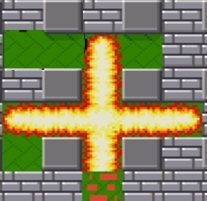
\includegraphics[scale=1]{explosao.jpg}
\caption{Explosão}
\label{bomba}
\end{figure}

\section{Requisitos de arte e áudio}
Para a arte do jogo será utilizado sprites buscadas do site tutsplus\footnote{http://gamedevelopment.tutsplus.com/articles/enjoy-these-totally-free-bomberman-inspired-sprites--gamedev-8541} , que disponibiliza de forma gratuita. Para o áudio será utilizado apenas sons ambiente que ainda não foram escolhidos.

\section{Cronograma de desenvolvimento}
O cronograma previsto para o desenvolvimento do Remake do Super Bomberaman 3 está expecificado na tabela \ref{cronograma}.
\begin{table}[ht]
\centering
\vspace{0.5cm}
\begin{tabular}{|c|c|}
\hline   
\hline   
Data & Descrição \\
\hline   
05/10 & Começo do trabalho  \\
09/10 & Documentos prontos  \\
14/10 & Sprites prontas e lógica do mapa funcionando  \\
16/10 & Comandos e movimentação do personagem  \\
19/10 & Entrega da documentação e do inicio do projeto  \\
23/10 & Monstros criados   \\
30/10 & Mais mapas prontos  \\
06/11 & Lógica da bomba e quebra dos blocos \\
13/11 & Lógica dos monstros aprimorada  \\
20/11 & Áudio nas fases \\
27/11 & Correção de possíveis problemas \\
07/12 & Entrega Final do jogo \\
\hline   
\hline   
\end{tabular}
\label{cronograma}
\caption{Cronograma}
\end{table}



\end{document}
